%\documentclass[a4paper]{article}
\documentclass[11pt]{extarticle}

\usepackage[utf8]{inputenc}
\usepackage{listings}
\usepackage{lipsum}
\usepackage{hyperref}
\usepackage{amssymb}
\usepackage[english]{babel}
\usepackage[numbered,framed]{matlab-prettifier}
\usepackage[useregional]{datetime2}
\usepackage{graphicx}

\lstset{
  style              = Matlab-editor,
  basicstyle         = \mlttfamily,
  escapechar         = ",
  mlshowsectionrules = true,
}

\title{\vspace{2cm}Elaborato di\\ \textbf{Calcolo Numerico}\\ Anno Accademico 2016/2017\vspace{1cm}}

\author{Gabriele Puliti - \texttt{5300140} - \href{mailto:gabriele.puliti@stud.unifi.it}{\textit{gabriele.puliti@stud.unifi.it}}
\and Luca Passaretta - \texttt{ } - \href{mailto: }{\textit{ }}}

\date{}

\addto\captionsenglish{\renewcommand{\contentsname}{Capitoli}}

\begin{document}

\maketitle

\begin{center}
\today{}
\end{center}

\newpage
\
\newpage

\tableofcontents
\newpage
\
\newpage

\section{\textbf{Capitolo 1}}
\subsection{Esercizio 1}
Sapendo che il metodo iterativo è convergente a \( x^* \) allora per definizione si ha:
 \[
	\lim_{k \to +\infty}\ x_k = x^*
\]
 inoltre per definizione di \( \Phi \) si calcola il limite:
\[
    \lim_{k \to +\infty} \Phi(x_k) = \lim_{k \to +\infty} x_{k+1} = x^*
\]
 infine ipotizzando che la funzione \( \Phi \) sia uniformemente continua, è possibile calcolare il limite:
\[
    \lim_{k \to +\infty} \Phi(x_k) = \Phi(\lim_{k \to +\infty} x_k) = \Phi(x^*)
\]
 dai due limiti si ha la tesi:
\[
    \Phi(x^*) = x^* 
\]
\subsection{Esercizio 2}
Dal momento che le variabili intere di 2 byte in Fortran vengono gestite in Modulo e Segno, la variabile \texttt{numero} inizializzata con:
\begin{verbatim}
integer*2 numero
\end{verbatim}
varia tra \( -32768 \leq \texttt{numero} \leq 32767 \) (\( - 2^{15} \leq \texttt{numero} \leq 2^{15} - 1 \)). \\ 
Durante la terza iterazione del primo ciclo for si arriva al valore massimo rappresentabile tramite gli interi a 2 byte; alla quarta iterazione si avrà quindi la somma del \texttt{numero} in modulo e segno:
\[
(32767)_{10}+(1)_{10} = (0111111111111111)_{2,MS} + (0000000000000001)_{2,MS} = 
\] \( 
= (1000000000000000)_{2,MS} = (-32768)_{10} 
\) \\ \\
Nel secondo ciclo for, durante la quinta iterazione, al \texttt{numero} viene sottratto 1:
\[
(-32768)_{10}-(1)_{10} = (1000000000000000)_{2,MS} - (0000000000000001)_{2,MS} = 
\] \( 
= (0111111111111111)_{2,MS} = (32767)_{10} 
\) \\ \\
Da cui si spiega l'output del codice.
\subsection{Esercizio 3}
Per definizione si ha che la precisione di macchina \(u\), per arrotondamento e' data da:
\[
u=\frac{1}{2} b ^{1-m}
\]
Se \(b=8, m=5\) si ha:
\[ 
u = \frac{1}{2}\cdot 8^{1-5} = \frac{1}{2}\cdot 8^{-4} = 1,2 \cdot 10^{-4} 
\]

\subsection{Esercizio 4}
Il seguente codice in Python
\lstinputlisting[language=Python]{cap_1/es4/es4.py}

restituisce questo output:

\begin{tabular}{l*{6}{c}r}
i & \( x_i \) & \( y_i \)  \\
\hline
1 & 1.05170918076  &  0.0517091807565 \\
2 & 1.00501670842  &  0.00501670841679 \\
3 & 1.00050016671  &  0.000500166708385 \\
4 & 1.00005000167  &  5.0001667141e-05 \\
5 & 1.00000500001  &  5.00000696491e-06 \\
6 & 1.00000049996  &  4.99962183653e-07 \\
7 & 1.00000004943  &  4.94336802603e-08 \\
8 & 0.999999993923  &  -6.07747097092e-09 \\
9 & 1.00000008274  &  8.27403709991e-08 \\
10 & 1.00000008274  &  8.27403709991e-08 \\
11 & 1.00000008274  &  8.27403709991e-08 \\
12 & 1.00008890058  &  8.8900582341e-05 \\

\end{tabular} \\

Graficando il contenuto della tabella su di un piano XY abbiamo che \\

\textbf{magari rendiamo piu carino il grafico ed aumentiamo la scala per le ultime iterazioni in cui la funzione oscilla tra e-8 e e-5}\\

\includegraphics[scale=0.4]{cap_1/es4/es4.png}

\subsection{Esercizio 5}
Tesi:\\
Sia f(x) una funzione sufficentemente regolare e h>0 una quantità ``piccola''\\
Ipotesi:\\
\[
\frac{f(x_0 + h) - f(x_0 + h)}{2h} = f'(x_0) + O(h^2)
\]
\[
\frac{f(x_0 + h) -2f(x_0) - f(x_0 + h)}{h^2} = f''(x_0) + O(h^2)
\]
Dimostrazione:\\
Sviluppiamo la funzione f(x) mediante il polinomio di taylor al secondo ordine\\
\[
f(x) = f(x_0) + (x-x_0)f'(x_0)+\frac{(x-x_0)^2}{2}f''(x_0) + O((x-x_0)^3)
\]
Sostituiamo \[x=(x_0 +h)\] e  \[x=(x_0-h)\]
\[
f((x_0 +h) = f(x_0) + hf'(x_0)+\frac{h^2}{2}f''(x_0) + O(h^3)
\]
\[
f((x_0 -h) = f(x_0) - hf'(x_0)+\frac{h^2}{2}f''(x_0) + O(h^3)
\]
Risostituendo  nel rapporto incrementale dell'ipotesi otteniamo:
\[
\frac{ f(x_0) + hf'(x_0)+\frac{h^2}{2}f''(x_0) + O(h^3) - f(x_0) - hf'(x_0)+\frac{h^2}{2}f''(x_0) + O(h^3)}{2h} = \frac{2hf'(x_0) + O(h^3)}{2h} =f'(x_0) + O(h^2)
\]

Per la seconda uguaglianza dell'ipotesi basterà applicare lo stesso procedimento con uno sviluppo di taylor al 3° ordine.

\subsection{Esercizio 6}
Il seguente codice \texttt{MATLAB}\\
\lstinputlisting[language=Matlab]{cap_1/es6/es6.m}
produce come output il seguente grafico:\\
\includegraphics[scale=0.7]{cap_1/es6/es6.png}\\
Con i>6 l'errore di convergenza è pari a \(10^{-10}\).
Per valori più grandi viene approssimato a 0 dal calcolatore.\\
Possiamo quindi prendere n=6 per ottenere un errore di convergenza pari a \(10^{-12}\)

\subsection{Esercizio 7}
Abbiamo che 
\( u=\frac{1}{2} b ^{1-m} \approx 4.66 \cdot 10^{-10} \), 
supponendo che la base sia \( b=2 \) otteniamo
\[
	m = 1 - log_2{(4.66 \cdot 10 ^{-10})} \approx 31.99
\]
Quindi necessitiamo di 32 cifre per la mantissa.
\subsection{Esercizio 8}
Sapendo che la mantissa in decimale è calcolabile tramite la funzione:
\begin{itemize}
\item \( m = 1- log_{10}{u} \) (troncamento) 
\item \( m = 1- log_{10}{(2\cdot u)} \) (arrotondamento)
\end{itemize}
e che la precisione di macchina assuma un valore accettabilmente piccolo in modo tale che il \(log_{10}{u} \approx 1\), cioè $0\leq u<1$, allora è possibile scrivere:
\begin{itemize}
\item \( m = 1 - log_{10}{u} \approx -log_{10}{u} \) (troncamento)
\item \( m = 1 - log_{10}{2u} = 1 - log_{10}{2} - log_{10}{u} \approx -log_{10}{u} \) (arrotondamento)
\end{itemize}
\subsection{Esercizio 9}
\lstinputlisting[language=Matlab]{cap_1/es9/es9.m}

\subsection{Esercizio 10}
I problemi del calcolo della radice e dell'elevamento a potenza sono sempre ben condizionati (k=1/2 e k=2).  Il problema critico è l'overflowper la somma. Per evitare questa criticità proponiamo questa soluzione:
Troviamo quindi il massimo dei due addendi:\\
\[
m = max\{|x|,|y|\} 
\]
\[
\sqrt{x^2 + y^2}
\]
Dividiamo entrambi i membri per il massimo
\[
\sqrt{m^2*(\frac{x}{m}^2 + \frac{y}{m}^2)}
\]
Portiamo fuori il massimo dalla radice
\[
m*\sqrt{\frac{x}{m}^2 + \frac{y}{m}^2}
\]
In questo modo eviteremo la problematica dell'overflow per la somma e il problema resterà sempre ben condizionato.
\subsection{Esercizio 11}
L'espressione aritmetica dei due algoritmi è:\\
\begin{itemize}
\item{1)} (x+y)+z = x+y+z 
\item{2)}  x+(y+z) = x+y+z 
\end{itemize}
Ne consegue che sono equivalenti
In aritmetica finita, invece, avremo:
\begin{itemize}
\item{1)} \( (x\oplus y)\oplus z = fl(fl(fl(x) + fl(y)) +fl(z)) = \)\\
\( =((x(1+\varepsilon_x) + y(1+\varepsilon_y))(1+\varepsilon_A) +z(1+\varepsilon_z))(1+\varepsilon_B) = \) \\
\[\varepsilon_R =\frac{(x(1+\varepsilon_x)(1+\varepsilon_A)(1+\varepsilon_B) + y(1+\varepsilon_y)(1+\varepsilon_A)(1+\varepsilon_B)+z(1+\varepsilon_z))(1+\varepsilon_B) -x-y-z}{z+y+z}     \]
prendo \( \varepsilon_M = max\{\varepsilon_x, \varepsilon_y, \varepsilon_z, \varepsilon_A, \varepsilon_B\}\)
\[\varepsilon_R \leq \frac{x(1+\varepsilon_M)^3 + y(1+\varepsilon_M)^3+z(1+\varepsilon_M)^2 -x-y-z}{z+y+z} = \]
\[ =  \frac{x(3\varepsilon_M + 3\varepsilon_M^2 +\varepsilon_M^3) + y(3\varepsilon_M + 3\varepsilon_M^2 +\varepsilon_M^3)+z(2\varepsilon_M + \varepsilon_M^2)}{z+y+z}    \]
Sapendo che \(\varepsilon_M \leq 1 \) posso affermare che \( \varepsilon_M \geq \varepsilon_M^2 \geq \varepsilon_M?3 \) ed effettuare un'altra minorazione

\[ \varepsilon_R \leq \frac{7x\varepsilon_M + 7y\varepsilon_M + 3z\varepsilon_M}{x+y+z} = \varepsilon_M(3+4\frac{x+y}{x+y+z}) \]

\item{2)}  \( x\oplus (y\oplus z) =fl(fl(x) +fl( fl(y) +fl(z)))     \) \\
Il procedimento sarà analogo a quello visto prima con lo scambio degli addendi al nominatore della frazione
\[ \varepsilon_R \leq \frac{7z\varepsilon_M + 7y\varepsilon_M + 3x\varepsilon_M}{x+y+z} = \varepsilon_M(3+4\frac{z+y}{x+y+z}) \]
\end{itemize}
\subsection{Esercizio 12}
Sapendo che il numero di condizionamento del problema è dato da:
\[
k =  \big| f'_{x}\cdot\frac{x}{f(x)} \big|
\]
Dato che la nostra funzione è $f(x) = \sqrt{x}$ allora la derivata è data da \newline $f'(x)=\frac{1}{2\cdot\sqrt{x}}$, sostituendo otteniamo:
\[
k = \big| \frac{1}{2\cdot\sqrt{x}}\cdot\frac{x}{\sqrt{x}} \big| = \big| \frac{1}{2} \big| = \frac{1}{2}
\]
Come volevamo.
\subsection{Esercizio 13}
\begin{flushleft}
Nella riga 11 abbiamo calcolato e restituito in output il valore interno al logaritmo $\big|3(1-\frac{4}{3})+1\big|$ che teoricamente è zero, invece si ottiene $2.220446049250313e-16 $. 
Si può vedere che il codice MatLab:
\lstinputlisting{cap_1/es13/es13.m}
calcola i valori della funzione ottenendo il grafico:
\begin{figure}[H]
\label{fes113}
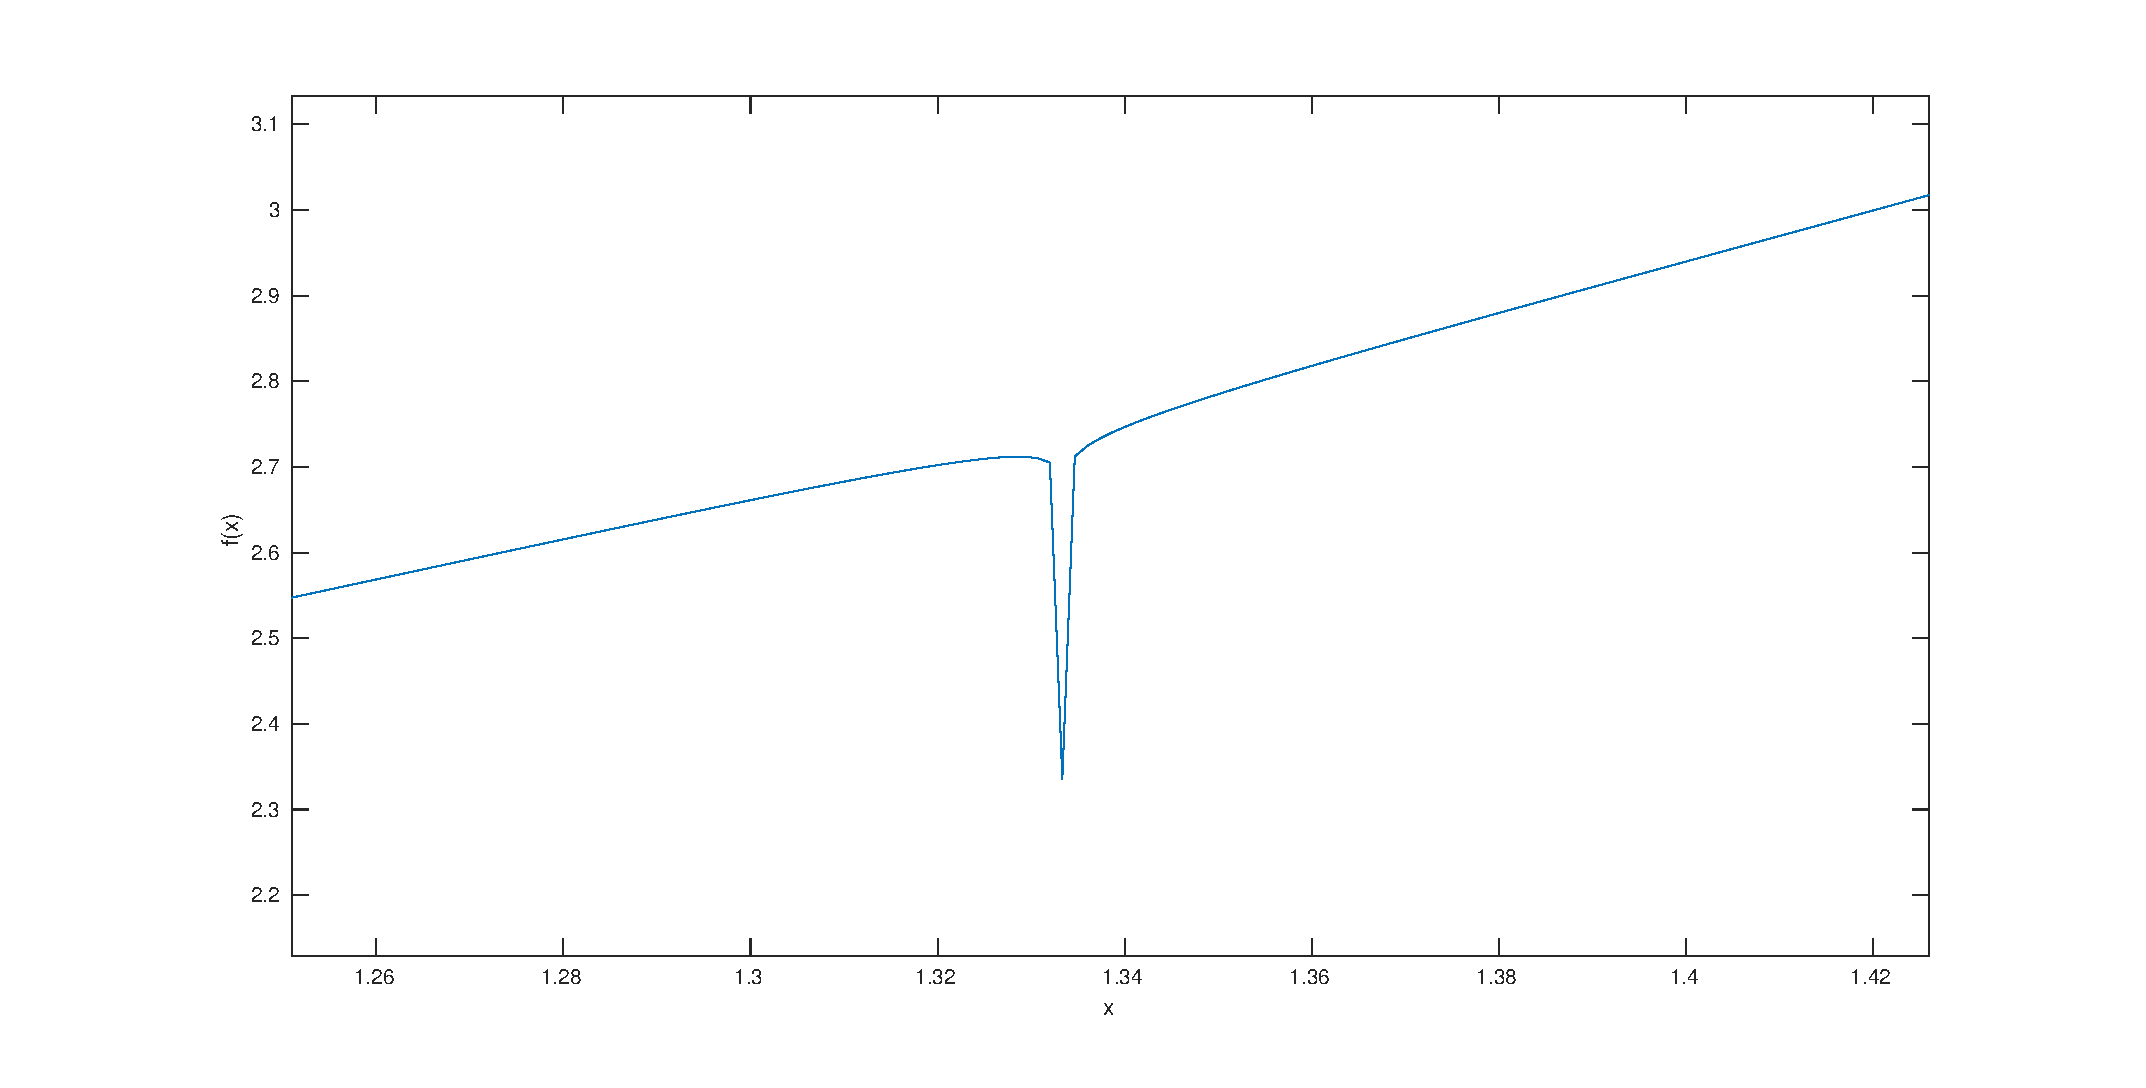
\includegraphics[width=450px]{plot/fes113}
\caption{\texttt{Plot MatLab della funzione $f(x)=\frac{ln(|3(1-x)+1|)}{80}+x^2+1$}}
\end{figure}
Si può notare che l'asintoto verticale in $x=\frac{4}{3}$ non viene rappresentato come tale. Il problema è che stiamo rappresentando dei numeri reali in un calcolatore, quindi la loro rappresentazione comporta delle approssimazioni. In questo caso infatti abbiamo il valore di $4/3$ che è un numero periodico, ma il calcolatore lo dovrà rappresentare con un numero di cifre finite causando un errore di rappresentazione che in questo caso risulta rilevante. Si allega sotto l'output del codice soprastante:
\includegraphics[width=10cm]{cap_1/es13/es113.png}
\end{flushleft}

\section{\textbf{Capitolo 2}}
\underline{Le funzioni usate nei codici seguenti sono in fondo al capitolo}
\subsection{Esercizio 1}

\lstinputlisting[language=Matlab]{cap_2/es1/es1.m}
La tabella delle approssimazioni è la seguente:
\begin{center}
\begin{tabular}{c|lc}
i & \( x_i \) \\
\hline
1 & 1.750000000000000e+00 \\
2 & 1.732142857142857e+00 \\
3 & 1.732050810014727e+00 \\
\end{tabular}\\
\end{center}

\subsection{Esercizio 2}
La radice da approssimare in questo caso è $\sqrt[n]{2}$ per gli $n=3,4,5$. Il codice MatLab corrispondente è il seguente:
\lstinputlisting[language=Matlab]{cap_2/es2/es2.m}
l'output corrispondente è:
\begin{center}
\begin{tabular}{c|c|c|c}
i & \( n=3 \) & \( n=4 \) & \( n=5\)\\
\hline
1 & 1.631784138709347e+00 & 1.771797299323380e+00 & 1.943788863498140e+00 \\
2 & 1.463411989089094e+00 & 1.463688102853308e+00 & 1.597060655491283e+00 \\
3 & 1.442554125137959e+00 & 1.336940995805593e+00 & 1.369877122538772e+00 \\
4 & 1.442249634601091e+00 & 1.316557487370408e+00 & 1.266284124539191e+00 \\
5 & 1.442249570307411e+00 & 1.316074279204018e+00 & 1.246387399421677e+00 \\
6 & ------------ & 1.316074012952573e+00 & 1.245731630753065e+00 \\
7 & ------------ & ------------ & 1.245730939616284e+00 \\
\end{tabular}
\end{center}
\subsection{Esercizio 3}
Per confrontare il metodo delle secanti con quello di Newton abbiamo creato il codice MatLab:
\lstinputlisting[language=Matlab]{cap_2/es3/es3.m}
I risultati ottenuti dall'utilizzo del metodo delle secanti sono: \newline
\\
\scalebox{0.7} {
\begin{tabular}{c|c|c|c|c}
i & metodo di Newton & metodo delle secanti & \big|newton-$\sqrt{2}$\big| & \big|secanti-$\sqrt{2}$\big|\\
\hline
1 & 1.750000000000000e+00 & 1.736842105263158e+00 & 3.357864376269049e-01 & 3.226285428900628e-01 \\
2 & 1.732142857142857e+00 & 1.732142857142857e+00 & 3.179292947697618e-01 & 3.179292947697618e-01 \\
3 & 1.732050810014727e+00 & 1.732050934706042e+00 & 3.178372476416318e-01 & 3.178373723329468e-01 \\
4 & --------- & 1.732050807572255e+00 & ------- & 3.178372451991598e-01\\
\end{tabular}
}
\\ \newline
Si nota dalla tabella che \( \big|newton-\sqrt{2}\big| \approx  \big|secanti-\sqrt{2}\big| \), cioè che l'ordine di grandezza dell'errore assoluto tra i due metodi è lo stesso. Si può quindi affermare che l'uso del metodo di Newton o del metodo delle secanti è equivalente.
\newpage
\subsection{Esercizio 4}
\lstinputlisting[language=Matlab]{cap_2/es4/es4.m}
Questo codice esegue i metodi di Newton, Newton modificato e Aitken per le funzioni date.
Questi sono gli output dei tre metodi numerici:\\
Funzione1:\\
\begin{tabular}{lc}
metodo & output \\
\hline
NewtonMod (m=1) & 3.014159265358980 \\
NewtonMod (m=10)& 3.141592653589793 \\
Aitken & 3.141592653589755 \\
\end{tabular}\\
Funzione2:\\
\begin{tabular}{lc}
metodo & output \\
\hline
NewtonMod (m=1) & 3.014571920744193 \\
NewtonMod (m=10)& 3.145719207441934 \\
Aitken & 3.137995613065127 \\
\end{tabular}\\

\subsection{Esercizio 5}
Il metodo di bisezione è applicabile in $f$ se è:
\begin{enumerate}
\item continua nell'intervallo $[a,b]$
\item $f(a)f(b)<0$
\end{enumerate}

\begin{flushleft}
il metodo di bisezione non è possibile utilizzarlo a causa della seconda condizione dato che $f_1(x)=(x-\pi)^{10}>0 \forall x$ e $f_2(x)=e^{2x}(x-\pi)^{10}>0 \forall x$ sono sempre positive quindi non è possibile stabilire un intervallo $[a,b]$ tale che $f(a)f(b)<0$, $\forall a,b \in \mathbb{R}$
\end{flushleft}
 


\subsection{Esercizio 6}
\lstinputlisting[language=Matlab]{cap_2/es6/es6.m}
\newpage
\subsection{Esercizio 7}
\lstinputlisting[language=Matlab]{cap_2/es7/es7.m}

I dati generati dall'esecuzione del codice sono esposti  nella seguente tabella

\begin{tabular}{l c r}

n & $tol_x$ & y \\
\hline
0 & $10^{-1}$ & 0.500000000000000 \\
7 & $10^{-2}$ & 0.488281250000000 \\
10 & $10^{-3}$ &  0.488769531250000 \\
13 & $10^{-4}$ & 0.488952636718750 \\
16 & $10^{-5}$ & 0.488945007324219 \\
20 & $10^{-6}$ & 0.488943576812744 \\
21 & $10^{-7}$ & 0.488943815231323 \\
26 & $10^{-8}$ & 0.488943792879581 \\
30 & $10^{-9}$ & 0.488943794276565 \\
32 & $10^{-10}$ & 0.488943794392981 \\
\hline
\end{tabular}


\newpage
\subsection{Esercizio 8}
\begin{flushleft}
Per determinare la radice della funzione data, abbiamo scritto il seguente script MatLab:
\lstinputlisting[language=Matlab]{cap_2/es8/es8.m}
Con risultato in output:
\newline
\includegraphics[width=150px]{cap_2/es8/es28.png}
\newline
Si può vedere che il metodo non converge per il punto iniziale $x0=0$, ma con punto iniziale diverso $x0=4$ il metodo converge. Questo significa che il metodo può convergere localmente. Dobbiamo quindi studiare la convergenza locale della funzione $f(x)$. Tale convergenza risulta essere garantita solo in un intorno della radice, in questo caso in un intorno di $\pi$. Essendo la funzione $f(x) = (x-\pi)\cdot e^{10\cdot x}$ la funzione di iterazione che definisce il metodo è determinata da:
\[
\Phi(x) = x-\frac{(x-\pi)\cdot e^{10\cdot x}}{e^{10\cdot x}\cdot (10\cdot x - 10 \cdot \pi + 1)} = x - \frac{(x-\pi)}{(10\cdot x - 10 \cdot \pi + 1)}
\]
Per convergere localmente si deve avere $\pi$ punto fisso della funzione di iterazione $\Phi(x)$. si ha infatti che:
\[
\Phi(\pi) = \pi - \frac{(\pi-\pi)}{(10\cdot \pi - 10 \cdot \pi + 1)} = \pi - 0 = \pi
\]
Questo conferma il fatto che la funzione $f(x)$ è convergente localmente in un intorno di $\pi$, confermando i risultati ottenuti dallo script precedente.
\end{flushleft}

\subsection{Funzioni MatLab Usate}
\subsubsection{Metodo Newton per $\sqrt{\alpha}$}
\lstinputlisting[language=Matlab]{cap_2/NewtonSqrt.m}
\subsubsection{Metodo Newton per $\sqrt[n]{\alpha}$}
\lstinputlisting[language=Matlab]{cap_2/NewtonSqrtN.m}
\subsubsection{Metodo delle secanti per $\sqrt[n]{\alpha}$}
\lstinputlisting[language=Matlab]{cap_2/SecSqrtN.m}
\subsubsection{Metodo di Newton Modificato}
\lstinputlisting[language=Matlab]{cap_2/NewtonMod.m}
\subsubsection{Metodo di accelerazione di Aitken}
\lstinputlisting[language=Matlab]{cap_2/Aitken.m}
\subsubsection{Metodo delle secanti}
\lstinputlisting[language=Matlab]{cap_2/secanti.m}
\subsubsection{Metodo della bisezione}
\lstinputlisting[language=Matlab]{cap_2/bisect.m}
\subsubsection{Metodo delle corde}
\lstinputlisting[language=Matlab]{cap_2/corde.m}
\newpage

\pagenumbering{roman}
\section{\textbf{Grafici}}
\subsection{Esercizio 1.4}
\begin{figure}[h]
\caption{Esercizio 1.4}
\label{fes14}
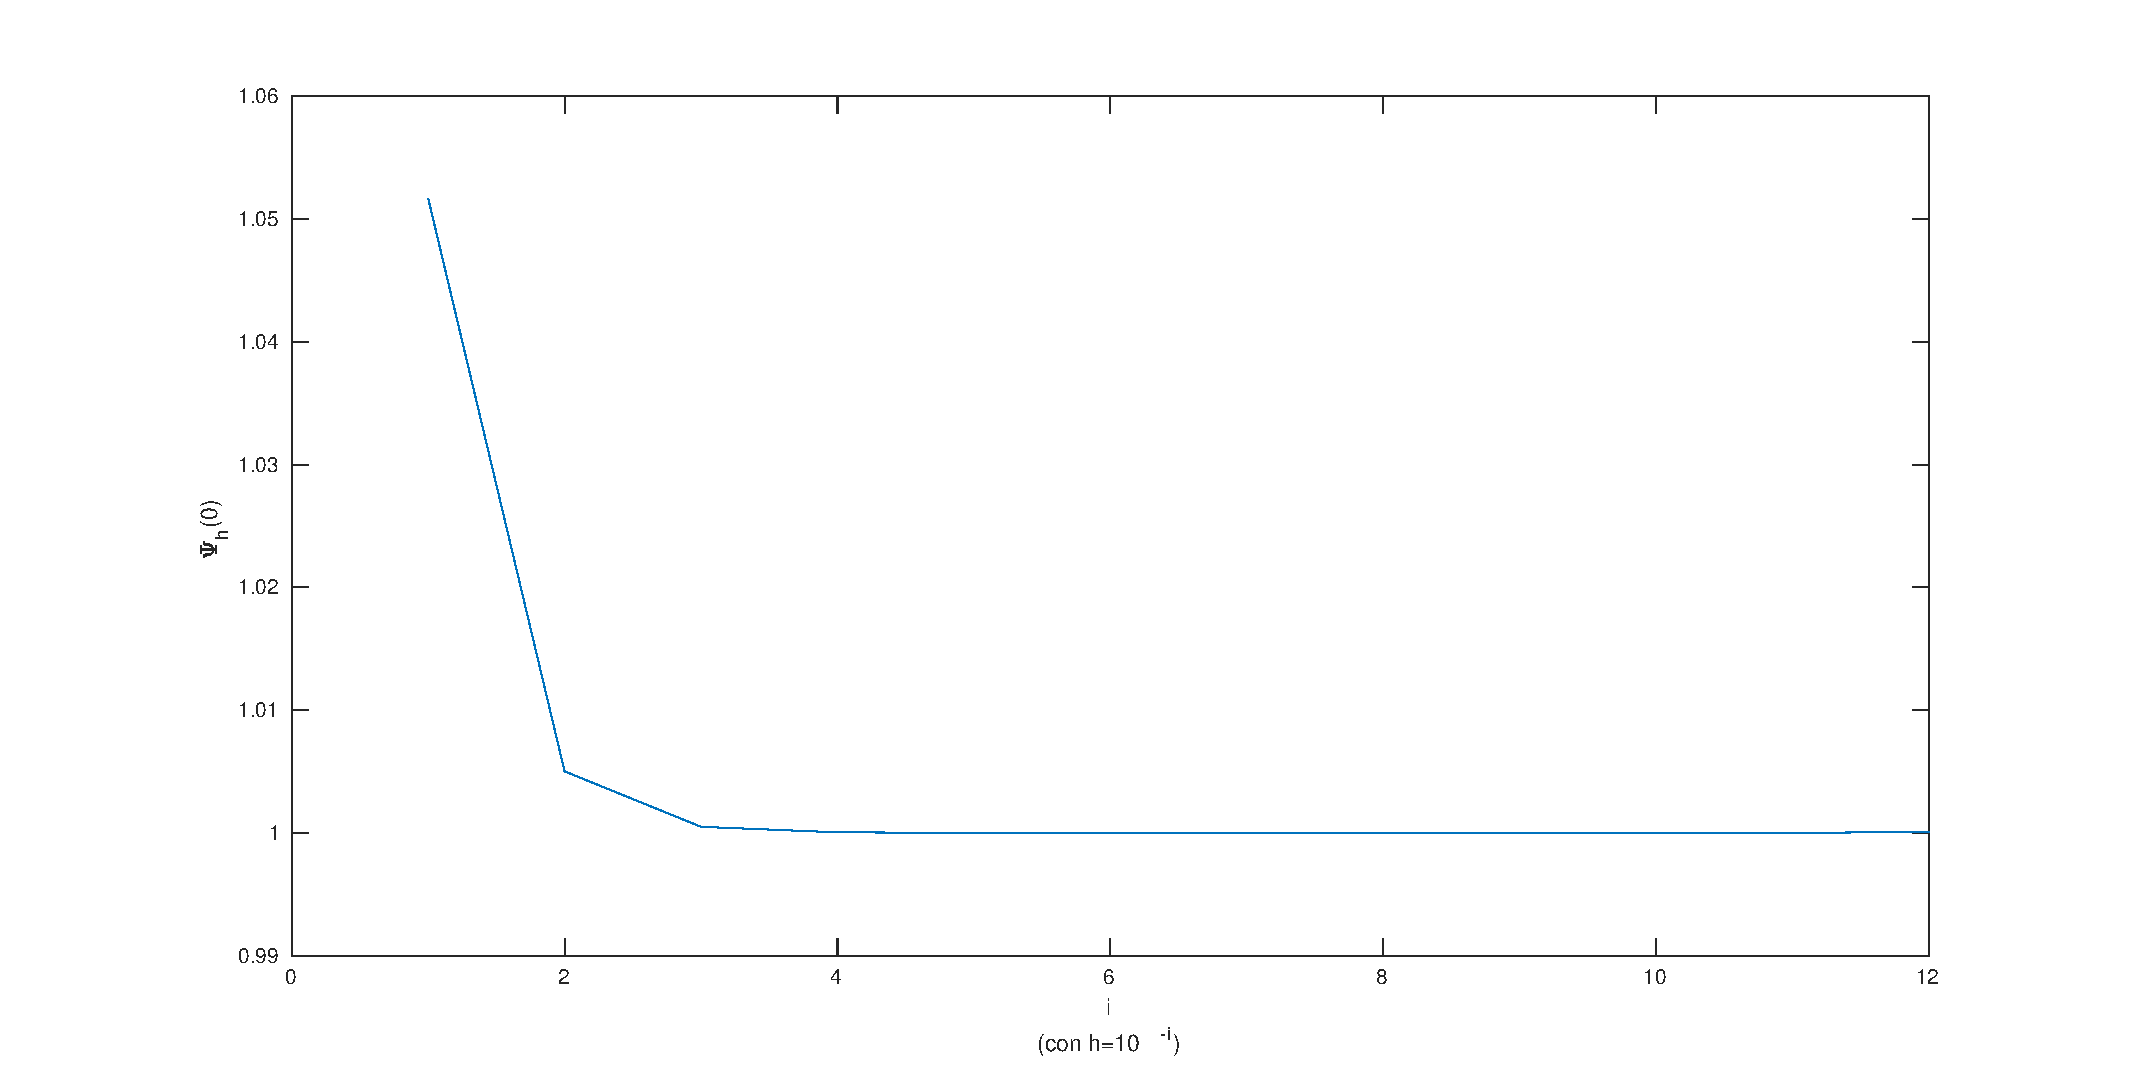
\includegraphics[width=\textwidth]{plot/fes14}
\end{figure}
\subsection{Esercizio 1.13}
\begin{figure}[h]
\caption{Esercizio 1.13}
\label{fes113}
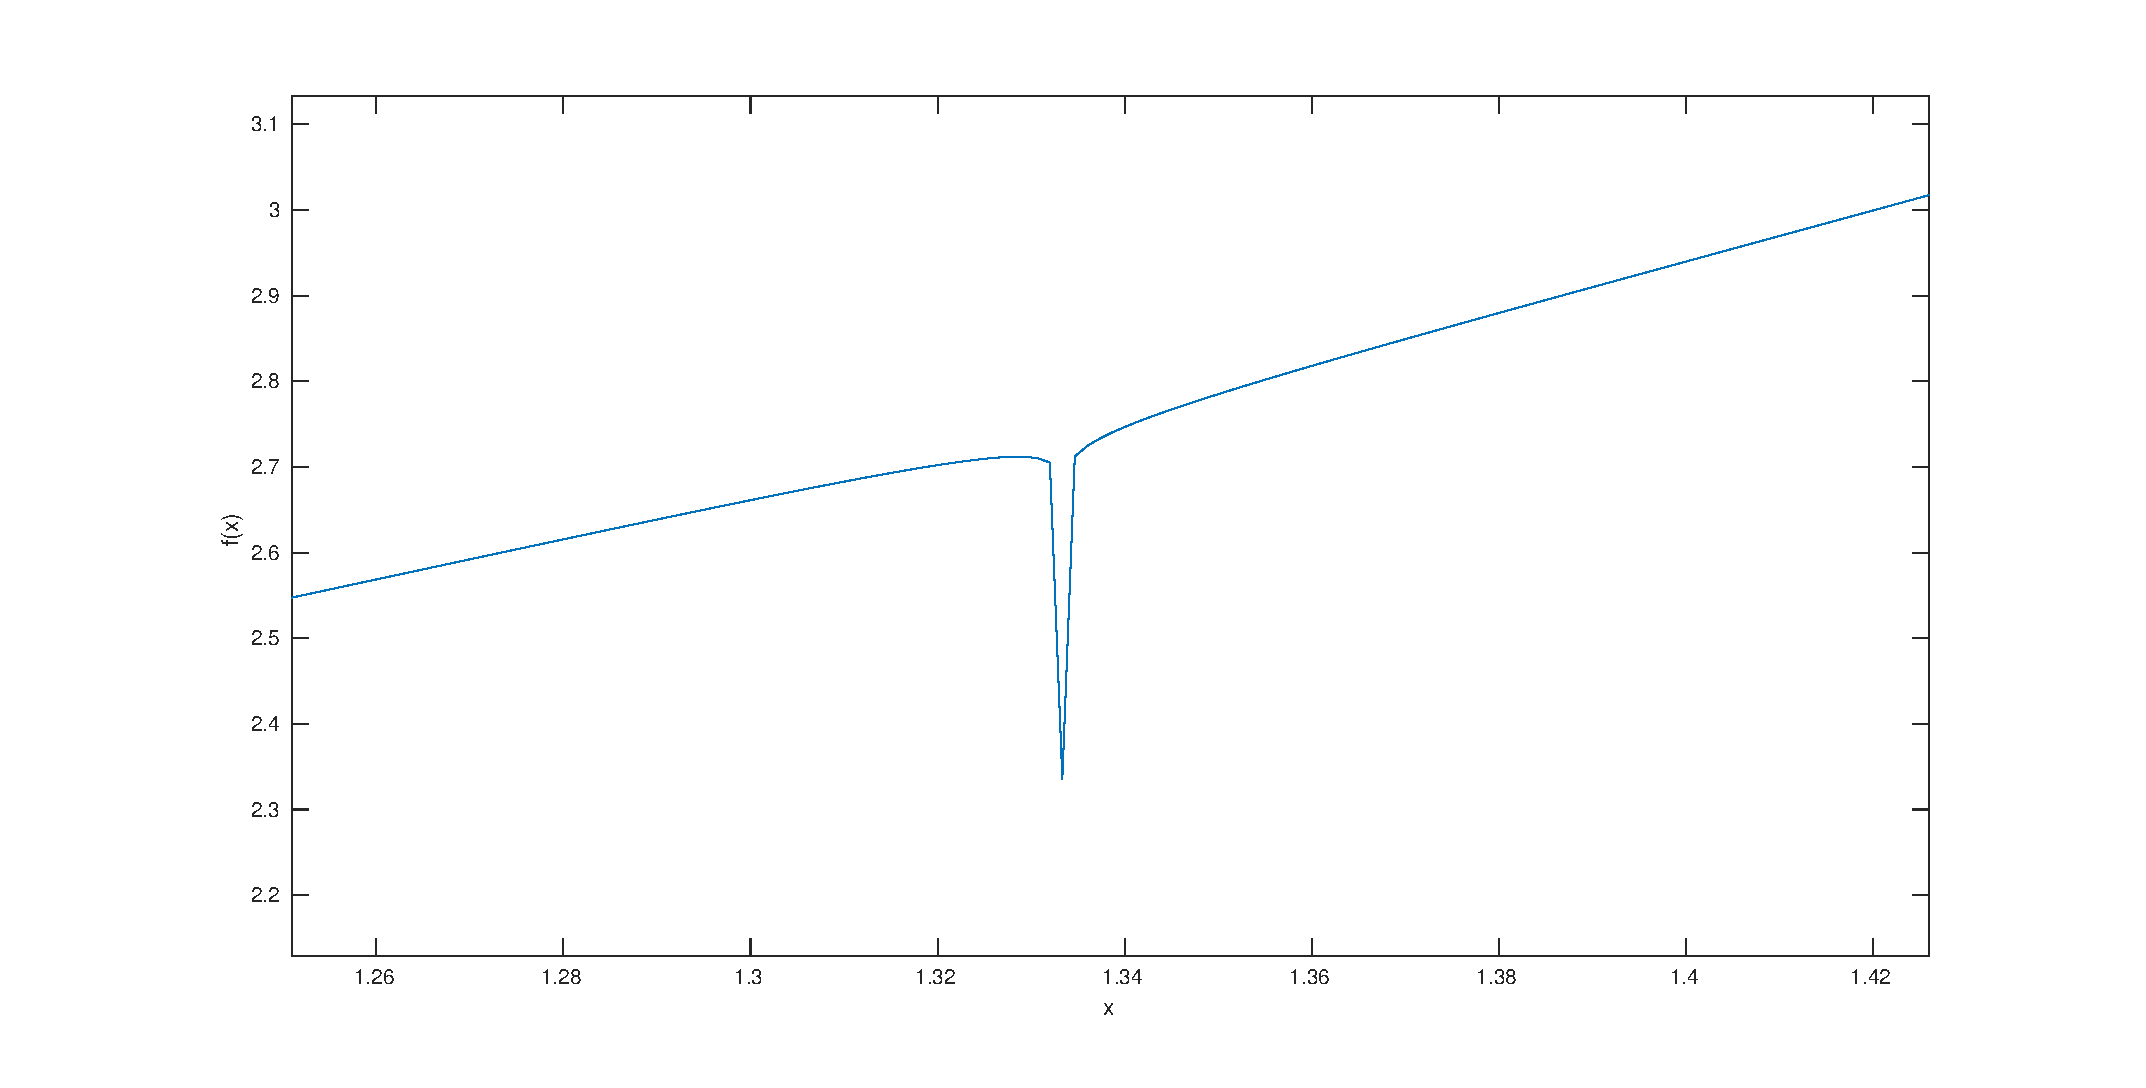
\includegraphics[width=\textwidth]{plot/fes113}
\end{figure}

\end{document}
